
\section{Нерекурсивный фильтр}
\label{sec:nerekurs}

\subsection{Расчёт фильтра}

\point Расчёт цифрового фильтра высоких частот (ФВЧ) со строго
линейной ФЧХ выполняется \textit{методом взвешивания}. Данный метод не
позволяет синтезировать оптимальные фильтры, но гораздо более удобен
для расчётов и даёт вполне приемлемые для практики результаты [1].


\point Исходные данные:

\begin{itemize}
\item тип фильтра~--- ФВЧ;
\item затухания в полосе задержания $a_0 = 45$ дБ;
\item характерные частоты фильтра $f_1 = 3000$ Гц;
\item ширина переходной полосы $\Delta f = 900$ Гц;
\item частота дискретизации $f_{\text{\textit{д}}} = 8000$ Гц;
\item мощность выходного шума квантования
    $\sigma^2_{\text{\textit{вых}}} = 5 \cdot 10^{-6}$.
\end{itemize}


\point Для упрощения обозначений удобно использовать нормализованную
шкалу относительных (или нормированных) частот:

\begin{equation}
  \label{eq:otn_freq}
  f_0 = \frac{f}{f_{\text{д}}},
\end{equation}

\begin{ESKDexplanation}
\item[где ] $f_{\text{д}}$~--- частота дискретизации;
\item $f_0$~--- относительное значение частоты;
\item $f$~--- абсолютное значение частоты.
\end{ESKDexplanation}

Таким образом, по формуле~(\ref{eq:otn_freq}):

\begin{gather*}
  f_{01} = \frac{f_1}{f_{\text{д}}} = \frac{3000}{8000} = 0{,}375;\\
  \Delta f_0 = \frac{\Delta f}{f_{\text{д}}} = \frac{900}{8000} = 0{,}113.
\end{gather*}


\point В соответствии с заданной величиной затухания в полосе
задерживания $a_0 = 45$ и графиками для окна Ланцоша, определяется
положительная постоянная~$L$ (см. формулу~(\ref{eq:lancosh})) и
\textit{порядок фильтра}~$N$:

\begin{gather*}
  (N-1)\Delta f_0 = 3;\\
  N = 27;\\
  L = 1{,}5.
\end{gather*}


\point \textit{Коэффициенты разложения в ряд Фурье} идеальной АЧХ
фильтра верхних частот:

\begin{gather}
  \nonumber
  h(0) = 1 - 2f_{01};\\
  \label{eq:koef_furier}
  h(k) = - \frac{\sin(2 \pi k f_{01})}{k \pi}.\\
  \nonumber
  k = - \frac{N}{2}, \ldots , \frac{N}{2} = -13, \ldots, 13.
\end{gather}

Результаты вычислений занесены в таблицу~\ref{tab:nonrekurs}
приложения~\ref{sec:AppendixA}.


\point Для уменьшения амплитуды пульсаций усечение импульсной реакции
производят с использованием весовой последовательности конечной длинны
$w(k)$, называемой временным окном. \textit{Весовые множители} $w(k)$
вычисляются из следующего выражения:

\begin{gather}
  \label{eq:lancosh}
  w(k) = \left[\frac{\displaystyle\sin\left(\frac{2\pi
          k}{N-1}\right)}{\displaystyle\frac{2\pi k}{N-1}}\right]^L,\\
  \nonumber
  k = -13, \ldots, 13,\\
  \nonumber
  L = 1{,}5.
\end{gather}

Результаты вычислений занесены в таблицу~\ref{tab:nonrekurs}
приложения~\ref{sec:AppendixA}.


\point На следующем этапе необходимо вычислить \textit{коэффициенты
  фильтра}. Процедура взвешивания сводится к умножению отсчётов $h(k)$
на соответствующие отсчёты $w(k)$ временного окна. Поэтому
коэффициенты ФВЧ вычисляются по формуле:

\begin{equation*}
  \hat h(k) = h(k) \cdot w(k).
\end{equation*}

Вычисленные значения коэффициентов фильтра представлены в
таблице~\ref{tab:nonrekurs} приложения~\ref{sec:AppendixA}.


\point Далее рассчитывается \textit{разрядность коэффициентов
  фильтра}. Коэффициенты каузального (физически реализуемого) фильтра
должны быть представимы конечным числом двоичных разрядов $N_k$.
Значение $N_K$ можно рассчитать по формуле:

\begin{align}
  \nonumber N_K & = \left[\log_2\left(\displaystyle
      \frac{\displaystyle 10 \cdot \frac{a_0}{20} \cdot
        \sqrt{\frac{2N-1}{3}}}{2}\right) \right]_{\text{Ц.Ч.}} + 1 =\\
  \nonumber & = \left[\log_2\left(\displaystyle \frac{\displaystyle 10
        \cdot \frac{45}{20} \cdot \sqrt{\frac{2 \cdot
            27-1}{3}}}{2}\right) \right]_{\text{Ц.Ч.}} + 1 = 7.
\end{align}


\point Далее по формуле~(\ref{eq:koef_okr}) вычисляются
\textit{округлённые значения коэффициентов фильтра}. Результаты
округления значений фильтра сведены в таблицу~\ref{tab:nonrekurs}
приложения~\ref{sec:AppendixA}.

\begin{equation}
  \label{eq:koef_okr}
  h_{\text{окр}} = 2^{-N_K} \cdot \left[h \cdot 2^{N_K}\right]_{\text{Ц.Ч.}}.
\end{equation}


\point Для практической реализации фильтра необходимо также оценить
\textit{разрядность входного} $S_{\text{вх}}$ и \textit{выходного}
$S_{\text{вых}}$ \textit{регистров фильтра}. Эти величины определяют
параметры шума квантования. Для определения величин $S_{\text{вх}}$ и
$S_{\text{вых}}$ можно пользоваться формулами:

\begin{gather*}
  S_{\text{вх}} = \left[ 0{,}5 \cdot \log_2\left(\frac{1{,}1 \sum_{l
          =0}^{N-1} \hat h^2(l)}{12 \sigma^2_{\text{вых}}} \right)
  \right]_{\text{Ц.Ч.}}
  + 1;\\
  S_{\text{вых.д}} = \left[0{,}5 \cdot \log_2\left( \frac{12N}{12
        \sigma^2_{\text{вых}} -2^{-2S_{\text{вх}}} \sum_{l=0}^{N-1}
        \hat
        h^2(l)}\right)\right]_{\text{Ц.Ч.}} + 1;\\
  S_{\text{вых.ц.}} = \left[0{,}5 \log_2 \sum_{l=0}^{N-1} \left|\hat
      h(l)\right|\right]_{\text{Ц.Ч.}};\\
  S_{\text{вых}} = S_{\text{вых.д}} + S_{\text{вых.ц.}}.
\end{gather*}

Выполнив необходимые вычисления, получаем:

\begin{gather*}
  S_{\text{вх}} = 7, \quad
  S_{\text{вых.д}} = 12,\quad
  S_{\text{вых.ц.}} = 0;\\
  S_{\text{вых}} = 12 + 0 = 12.
\end{gather*}

\subsection{АЧХ фильтра}

Комплексную частотную характеристику (КЧХ) нерекурсивного цифрового
фильтра можно определить из следующего соотношения:

\begin{equation*}
  H(e^{j\omega_0}) = \sum_{K=0}^{N-1}h(k) \cdot e^{-j\omega_0k},
\end{equation*}

\begin{ESKDexplanation}
\item[где ] $\omega_0$~--- круговая нормированная частота;
\item $N$~--- порядок фильтра.
\end{ESKDexplanation}

АЧХ представляет собой абсолютное значение от КЧХ. Модуль комплексного
числа можно определить как квадратный корень из суммы квадратов
вещественной и мнимой частей:

\begin{equation*}
\left|H(e^{j\omega_0}) \right| = \sqrt{\text{Re}^2H(e^{j\omega_0k}) + \text{Im}^2H(e^{j\omega_0k})}.
\end{equation*}

Используя формулу Эйлера:

\begin{equation*}
  e^{j\omega_0} = \cos\omega_0 + j \sin\omega_0,
\end{equation*}

записывается конечная формула для расчёта АЧХ нерекурсивного фильтра.

\begin{equation*}
   \left|H(e^{j\omega_0})\right| = \sqrt{\left[\sum_{k =
        -\frac{N-1}{2}}^{k =
        \frac{N-1}{2}}h(k)\cos(k\omega_0)\right]^2 + \left[\sum_{k =
        -\frac{N-1}{2}}^{k =
        \frac{N-1}{2}}h(k)\sin(k\omega_0)\right]^2}.
\end{equation*}

Для вычисления АЧХ нерекурсивного фильтра, необходимо оценить её на
главном значении периода. Для этого вычисляется дискретное
преобразование Фурье (ДПФ) этой функции.

\begin{figure}[h!]
  \label{f:1}
  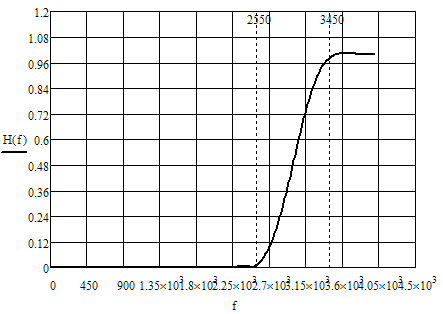
\includegraphics{ACH}
  \caption{АЧХ синтезированного нерекурсивного фильтра верхних частот}
\end{figure}

Для более удобного сопоставления полученных частотных характеристик с
требованиями технического задания, целесообразно значения АЧХ выразить
в логарифмических единицах:

\begin{equation*}
  a_0 = -20 \lg\left|H(e^{j \omega_0})\right|.
\end{equation*}

Для получения требуемой характеристики величина $N$ была увеличена до 14.

\begin{figure}[h!]
  \label{f:2}
  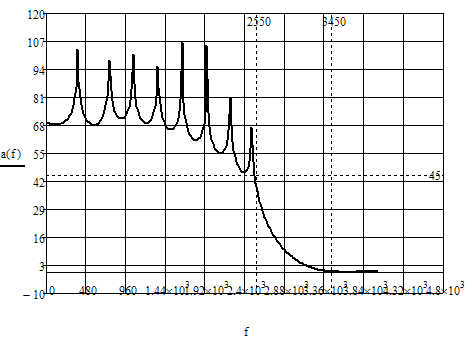
\includegraphics{LACH}
  \caption{ЛАЧХ синтезированного фильтра}
\end{figure}


Из графика представленного на рисунке~\ref{f:2} видно, что АЧХ синтезируемого
фильтра удовлетворяет требованиям технического задания. Это следует из
того, что на частоте 2550 Гц затухание соответствует 45 дБ.

\subsection{Структурная схема фильтра}

Структурная схема нерекурсивного цифрового фильтра приведена на 
рисунке

\newpage

\section{Рекурсивный фильтр}
\label{sec:rekurs}

\subsection{Расчёт фильтра}

\point Наиболее распространённым и простым методом синтеза для
стандартных частотно-избирательных фильтров является \textit{метод билинейного
преобразования} передаточной функции $K(P)$ аналогового фильтра-прототипа
(АФ) в соответствующую передаточную функцию $H(z)$ цифрового
рекурсивного фильтра (ЦРФ) [1].

\point Исходные данные:

\begin{itemize}
\item тип фильтра, характер аппроксимации~--- ППФ, Чебышева;
\item затухание в полосе задержания $a_0 = 40$ дБ;
\item верхняя граница затухания в полосе пропускания $\Delta a =$~0{,}8~дБ;
\item характерные частоты фильтра $f_{11} = 900$ Гц, $f_{12} = 1800$
  Гц, $f_{21} = 500$ Гц, $f_{22} = 2200$ Гц;
\item частота дискретизации $f_{\text{\textit{д}}} = 4800$ Гц;
\item мощность выходного шума квантования
  $\sigma^2_{\text{\textit{вых}}} = 10^{-5}$.
\end{itemize}

\point Согласно формуле~(\ref{eq:otn_freq}) \textit{относительные значения
характерных частот} фильта:

\begin{gather*}
  f_{011} = 0{,}1875;\\
  f_{012} = 0{,}3750;\\
  f_{021} = 0{,}1042;\\
  f_{022} = 0{,}4583.
\end{gather*}

\point По формулам, описывающим обобщённое билинейное преобразование,
определяются значения параметров $\gamma$ и $\alpha$, а также
\textit{граничная частота} $\Omega_k$ нормированного аналогового
фильтра-прототипа:

\begin{gather*}
  \gamma = \ctg \left[\pi (f_{012} - f_{011})\right] = 1{,}947;\\
  \alpha = \frac{\cos\left[\pi (f_{012} + f_{011})
    \right]}{\cos\left[\pi (f_{012} - f_{011}) \right]} = -0{,}235;\\
  \Omega'_k = \gamma \frac{\alpha - cos(2\pi f_{021})}{\sin(2\pi
    f_{021})} = -2{,}527;\\
  \Omega''_k = \gamma \frac{\alpha - cos(2\pi f_{022})}{\sin(2\pi
    f_{022})} = 4{,}229;\\
  \Omega_k = \text{min}\bigl(|\Omega'_k|,|\Omega''_k|\bigr) = 2{,}527.
\end{gather*}


\point Следующим этапом является определение \textit{передаточной
  функции} аналогового фильтра-прототипа для полосового фильтра с
аппроксимацией Чебышева рассчитали по справочнику [3]. С его помощью
определяем:

\begin{itemize}
\item модуль коэффициента отражения $|P| = 25\%$;
\item вспомогательный параметр $L = 0{,}05$
\item \textit{порядок фильтра} $n = 5$;
\item передаточная функция:
  \begin{equation*}
    K(P) = \frac{1}{C \cdot \prod_{i =1}^2 \left[P^2 - 2a_iP + a_i^2
        + b_i^2\right]},
  \end{equation*}
  \begin{ESKDexplanation}
  \item[где ] $C = 4{,}1311822$;
  \item $a_1 = 0{,}3434291432$;
  \item $a_2 = 0{,}1311782600$;
  \item $b_1 = 0{,}6385527983$;
  \item $b_2 = 1{,}0332001312$.
  \end{ESKDexplanation}
\end{itemize}

\point Чтобы избежать трудоёмкого расчёта уравнения 4-го порядка,
разложили передаточную функцию фильтра-прототипа в виде произведений
полиномов 1-го порядка по степеням Р [2]. Для этого следует расписать
полиномы в виде:

\begin{equation*}
  P^2 + a_1P + a_2 = (P-P_1)(P-P_2),
\end{equation*}
\begin{ESKDexplanation}
\item[где ] $P_1$ и $P_2$~--- комплексные корни квадратного уравнения;
\item $a_1$ и $a_2$~--- действительные коэффициенты.
\end{ESKDexplanation}

Получаем \textit{значения полюсов}:

\begin{gather*}
  p_1 = -0{,}342 - 0{,}639;\\
  p_2 = 0{,}343 + 0{,}639;\\
  p_3 = -0{,}131 - 1{,}033;\\
  p_4 = -0{,}424502.
\end{gather*}

\point Затем осуществляем подстановку:

\begin{equation*}
  P = \rightarrow \gamma \frac{1 - 2 \alpha z^{-1}+z^{-2}}{1-z^{-2}}.
\end{equation*}

Затем умножаем числитель и знаменатель дроби на $z^2$. После
преобразований получаем выражение вида:

\begin{equation*}
  H(z) = \frac{A(z^2 - 1)^n}{\displaystyle \prod_{i=1}^n\left[(\gamma - p_i)z^2 -
      2\alpha \gamma z + (\gamma + p_i)\right]}.
\end{equation*}

Получаем корни

%%% Local Variables: 
%%% mode: latex
%%% TeX-master: "../TermWork_TES"
%%% End: 
